\documentclass{foi}
\usepackage[utf8]{inputenc}
\usepackage{lipsum}
\usepackage{float}
\usepackage{hyperref}
\usepackage{enumitem}

\DeclareUnicodeCharacter{0140}{l}
\vrstaRada{\diplomski} % \diplomski
\title{Izrada komponente za detekciju označenih odgovora na pismenim ispitima}
\author{Filip Milohanović}
\spolStudenta{\musko} % \zensko ili \musko
\mentor{Marko Mijač}
\spolMentora{\musko} % \zensko ili \musko
\godina{2025}
\mjesec{lipanj}
\date{2025}
%\status{redoviti}
\jmbag{0016148270 }
\smjer{Informacijsko i programsko inženjerstvo} % (ili Poslovni sustavi, Ekonomika poduzetništva, Primjena informacijske tehnologije u poslovanju, Informacijsko i programsko inženjerstvo, Baze podataka i baze znanja, Organizacija poslovnih sustava, Informatika u obrazovanju)
\titulaProfesora{Doc. dr. sc.}

\sazetak{Opsega od 100 do 300 riječi. Sažetak upućuje na temu rada, ukratko se iznosi čime se rad bavi, teorijsko-metodološka polazišta, glavne teze i smjer rada te zaključci.}

\kljucneRijeci{riječ; riječ; ...riječ; Obuhvaća 7+/-2 ključna pojma koji su glavni predmet rasprave u radu.}

\begin{document}

\maketitle

\tableofcontents

\pagestyle{plain}
\chapter{Uvod}

U današnjem obrazovnom sustavu nastavnici provode jako puno vremena na radnim zadacima koji ne podižu kvalitetu obrazovanja već su administrativni i često repetitivni poslovi. Jedan od tih zadataka je ocjenjivanje ispita, pogotovo ako se radi o velikoj količini pristupnika testu. Kod testova s izrazito velikom količinom pristupnika se zato koriste ispiti koji uključuju list za odgovore što olakšava ocjenjivanje. Time se značajno ubrzava cijeli proces ocjenjivanja pošto nije potrebno čitati odgovore koji su u različitim formatima i potencijalno na više stranica, ali i dalje ostaje repetitivni dio posla koji uključuje usporedbu odgovora s rješenjima. Kroz ovaj rad bit će prikazana softverska komponenta otvorenog koda koja rješava ovaj problem tako da naspram slike detektira označene odgovore i ocjenjuje ispit.

Kroz ovaj rad istražuje se razne metode za detektiranje označenih odgovora s ciljem izrade komponente visoke preciznosti, prateći metodologiju znanstvenog oblikovanja.

\chapter{Metode i tehnike rada}

S obzirom na to da se radi o temi koja uključuje obradu slike, što zahtijeva opsežno istraživanja, manipulaciju parametrima i testiranje pristupa odlučeno je koristiti inkrementalan pristup razvoju. Prije same izrade rješenja, provedena je minimalno potrebna količina istraživanja, a zatim se ostatak istraživanja odvijao paralelno s razvojem.

Iterativni razvoj rješenja može se podijeliti u pretprocesiranje, izdvajanje relevantnih obilježja slike i na kraju ocjenjivanje testa. Jedna od najvažnijih tehnika tijekom razvoja bila je  vizualizacija svakog koraka obrade slike. To je omogućilo izravan uvid u status i smjer razvoja. Od samog početka omogućen je uvid u mane i prednosti korištenih metoda. Ovo je značajno doprinijelo definiranju budućih razvojnih koraka, poput  dodatnog istraživanja, promjene pristupa i sl. 

Da bi sama vizualizacija bila što učinkovitija korišteno je više različitih ulaznih slika matrice odgovora slikanih u različitim uvjetima. To je omogućilo verifikaciju funkcionalnosti dijelova rješenja na različitim ulaznim podacima od samog početka razvoja, što je značilo da na kraju projekta nije bilo potrebno pokrivati rubne slučajeve jer je rješenje bilo dizajnirano da ih pokriva od početka.

Rješenje je izrađeno pomoću .NET tehnologije i C\# programskog jezika u obliku biblioteke, što omogućuje drugim rješenjima jednostavnu integraciju koristeći .dll. 

Kroz ovaj rad nije bio cilj razviti vlastitu biblioteku za računalni vid, korištena je jedna od  postojećih biblioteka otvorenog koda. EmguCv je odabran pošto se radi o .NET omotaču za jednu od najpopularnijih biblioteka za računalni vid OpenCV. Osim toga, rješenje omogućuje korisnicima da koriste alternativnu biblioteku s uvjetom da izrade svoju implementaciju odgovarajućih metoda.

\chapter{Razrada teme}

Kroz teoretski dio rada predočit će se cijeli proces detekcije odgovora na pismenim ispitima koristeći obradu slike pomoću računalnog vida. Analizirat će postojeća rješenja ovog problema koja koriste računalni vidi i alternativne pristupe. 

Svim ti pristupi imaju isti cilj, a to je izvlačenje relevantnih podataka iz slike, a zatim kreće obrada tih podataka. U kontekstu ovog rada to bi značilo da se iz slike moraju izvući podaci o označenim odgovorima za određeno pitanje te se ti podaci uspoređuju s listom točnih odgovora. 

\section{Digitalna slika }

Za početak važno je razumjeti što su to digitalne slike i koje sve informacije one sadrže. Digitalna slika je zapravo računalna datoteka koja reprezentira fotografiju pomoću piksela. Piksel je zapravo najmanji element slike koji je reprezentiran s 3 kanala boja: Crvena (R), zelena (G), plava (B) u RGB modelu. Postoje i drugi kanali boja sli za potrebe ovog rada fokus će biti RGB modelu.  \cite{DigitalnaSlika}.

Sama boja piksela se određuje kombinacijom vrijednosti iz RGB kanala. Dok je sam broj mogućih boja određen brojem bitova koju svaki RGB kanal može poprimiti. Taj koncept se još naziva dubinom boje (eng. color depth). Na primjer, 24-bitna slika može poprimiti do 16,777,216 unikatnih boja pošto svaki kanal ima 8 bitova \cite{DigitalnaSlika}:

\[
\text{Broj boja} = 2^{8} \times 2^{8} \times 2^{8} = 2^{24} = 16,777,216
\]

S pomoću piksela se također može definirati veličinu slike to jest rezolucija. Rezolucija je sveukupan broj piksela koje neka slika sadrži i izražava se množenjem širine slike s visinom slike npr. $1920 \times $1080. Obično veća rezolucija znači više detalja na slici. Što se više detalja nalazi na slici to su bolje šanse za izvući korisne informacije sa slike. No naravno da rezolucija sama ne određuje kvalitetu digitalne slike, već veliku ulogu igraju i fizički uvjeti u kojima je slika izrađena. Pod to spada osvjetljenje, čistoća kamere, kvaliteta senzora i sl.

\subsection{Slike u boji}
Većina digitalnih slika koje ljudi danas izrađuju su slike u boju te sadrže sva 3 kanala boje. Za razumijevanje ovog rada potrebno je razumjeti kakve informacije sadrži pojedini kanal boje. Svaki kanal predstavlja jednu primarnu boju poput crvene, zelene ili plave. I svaki piksel poprima određenu vrijednost za svaki kanal ovisno o kombinaciji bitova. Za 24-bitnu sliku svaki kanal ima 8 bitova to jest 256 mogućih vrijednosti. 

To znači da u svakom kanalu postoji vrijednost od 0 do 255 koja definira jačinu svjetlosti za tu primarnu boju. Nula bi značila kompletno crna boja dok bi 255 bila potpuno osvijetljena primarna boja ovisno o kojem se kanalu radi. Kombinacijom tih 3 kanala se zapravo dobivaju međuboje i time se stvara konačni izgled slike. \cite{GrayscaleSlika}.

\begin{figure}[h!]
    \centering
    \includegraphics[width=1.0\linewidth]{slike/Color_chanell_separation.png}
    \caption{Prikaz slike u boji i pripadajućih kanala boja u RGB modelu (vlastita izrada)}
    \label{fig:channels}
\end{figure}

Kao što je prikazano na slici, kanali boja prikazani su kao slike čiji pikseli poprimaju boje samo crnu, bijelu i nijanse sive boje, takozvane sive slike. Također kanali se ponekad znaju vizualizirati pomoću primarne boje kanala kojeg reprezentiraju, ali sami podaci koje digitalna slika sadrži su uvijek jednaki, jedino način njihove vizualizacije varira. 

\subsection{Sive slike}

Sive slike (\textit{eng. grayscale}) su poseban tip digitalnih slika koji ima samo jedan kanal boja. U tom kanalu vrijednosti piksela reprezentira svjetlinu piksela. Vizualizacija takvih slika poprima boje od bijele do crne uključujući nijanse sive. Na primjer za sliku sa dubinom boja od 8 bitova, nula bi predstavljala crnu boju, 255 bijelu, a vrijednosti između nijanse sive \cite{GrayscaleSlika}.

Sive slike su jedan od važnijih koncepata obrade slike i računalnog vida. One su zapravo baza mnogih algoritama za procesiranje slika. Često se koriste kao prvi korak obrade. Izrazito su korisne za detekciju rubova, segmentaciju slike, prepoznavanje uzorak i slično \cite{Grayscale2}. Kroz rad će se detaljnije prikazati njihova važnost i uloga u kontekstu detektiranja označenih odgovora na pismenim ispitima. 

\begin{figure}[H]
    \centering
    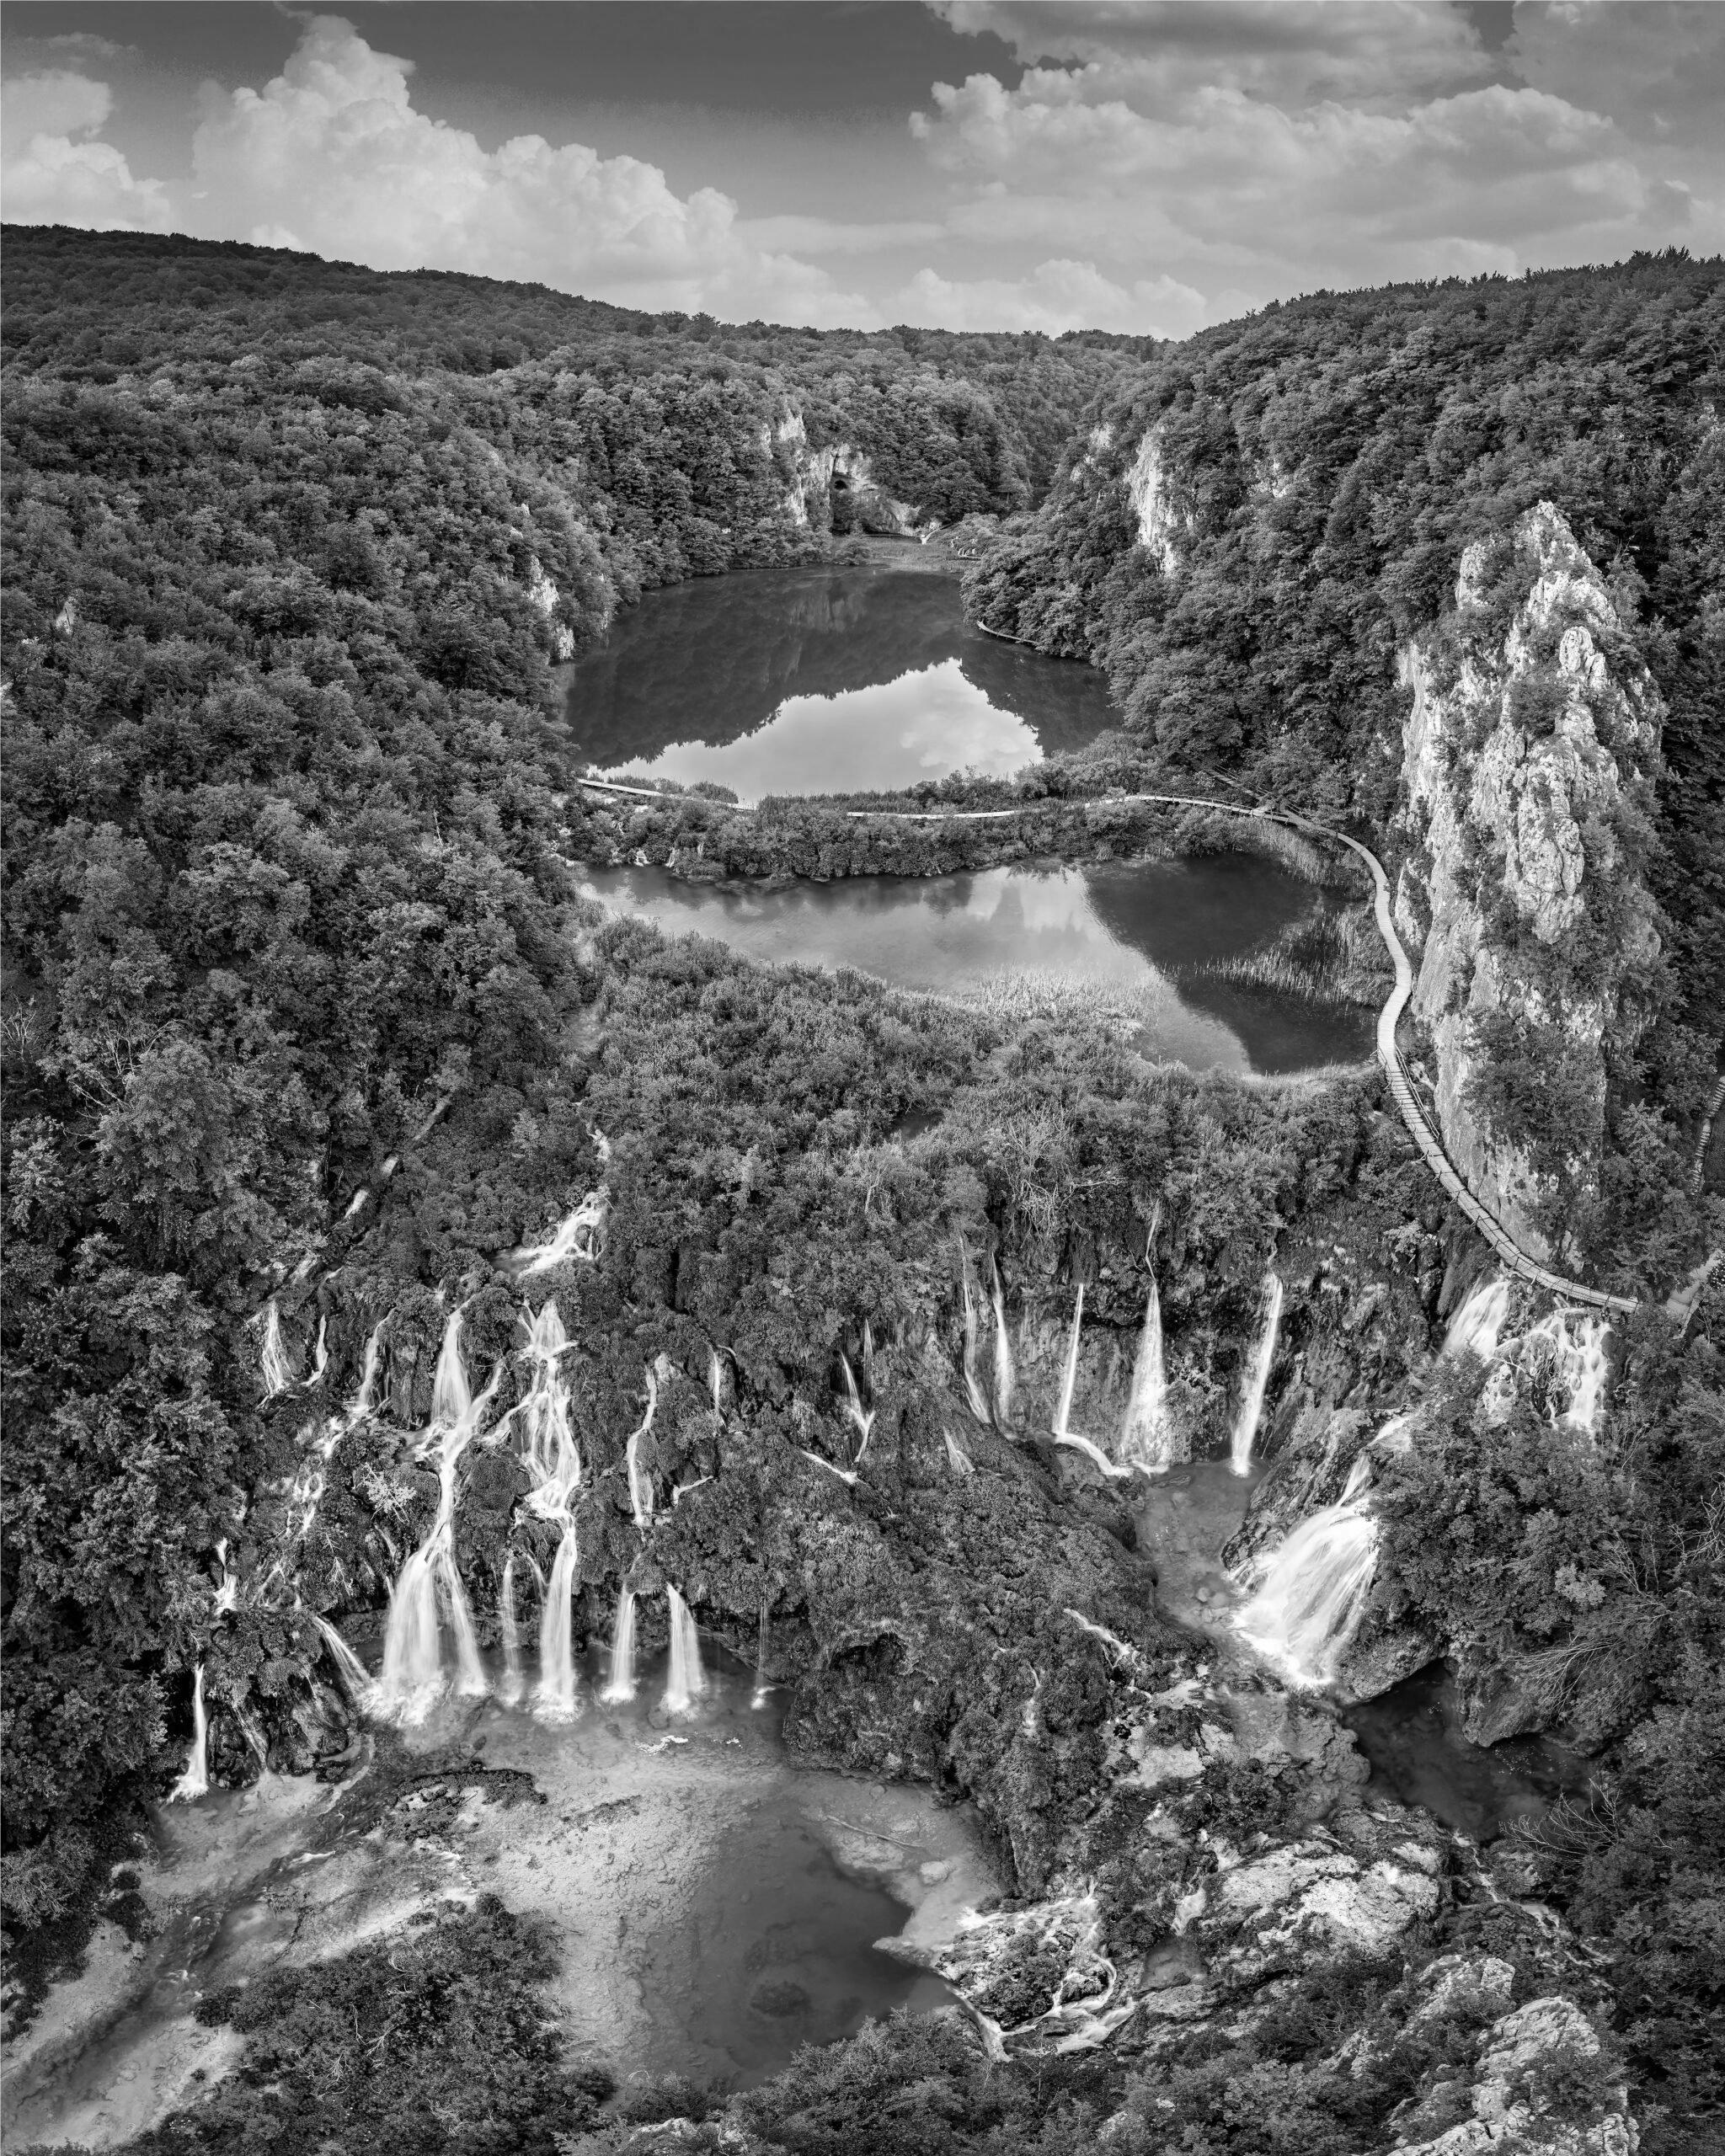
\includegraphics[width=0.7\linewidth]{slike/Grayscale.jpeg}
    \caption{Prikaz sive slike (vlastita izrada)}
\end{figure}

Na priloženoj sivoj slici se također može vidjeti da je različita od sivih slika kanala prikazanih na \hyperref[fig:channels]{slici 1}. To je zato što se kod pretvorbe slike u boji u sivu sliku uzimaju u obzir vrijednosti piksela za sva 3 kanala prema formuli:

{\large
\[
    I_{\text{gray}}(x, y) = 0.299 \cdot R(x, y) + 0.587 \cdot G(x, y) + 0.114 \cdot B(x, y)\text{\cite{Grayscale2}}
\]
}


\subsection{Binarne slike}

Osim slika u boji i sivih slika također postoje i binarne slike. Binarne slike su tip slika gdje piksel može imati samo dvije moguću vrijednosti 0 i 1 od kud im dolazi i naziv. Binarne slike sadrže puno manje informacija od ostalih tipova slika, ali isto tako smanjuju kompleksnost same slike i omogućuju fokusiranje na važne značajke slike. Baš zbog toga se jako često koriste kod obrada slika koristeći računalni vid \cite{BinarySlika}.

\begin{figure}[H]
    \centering
    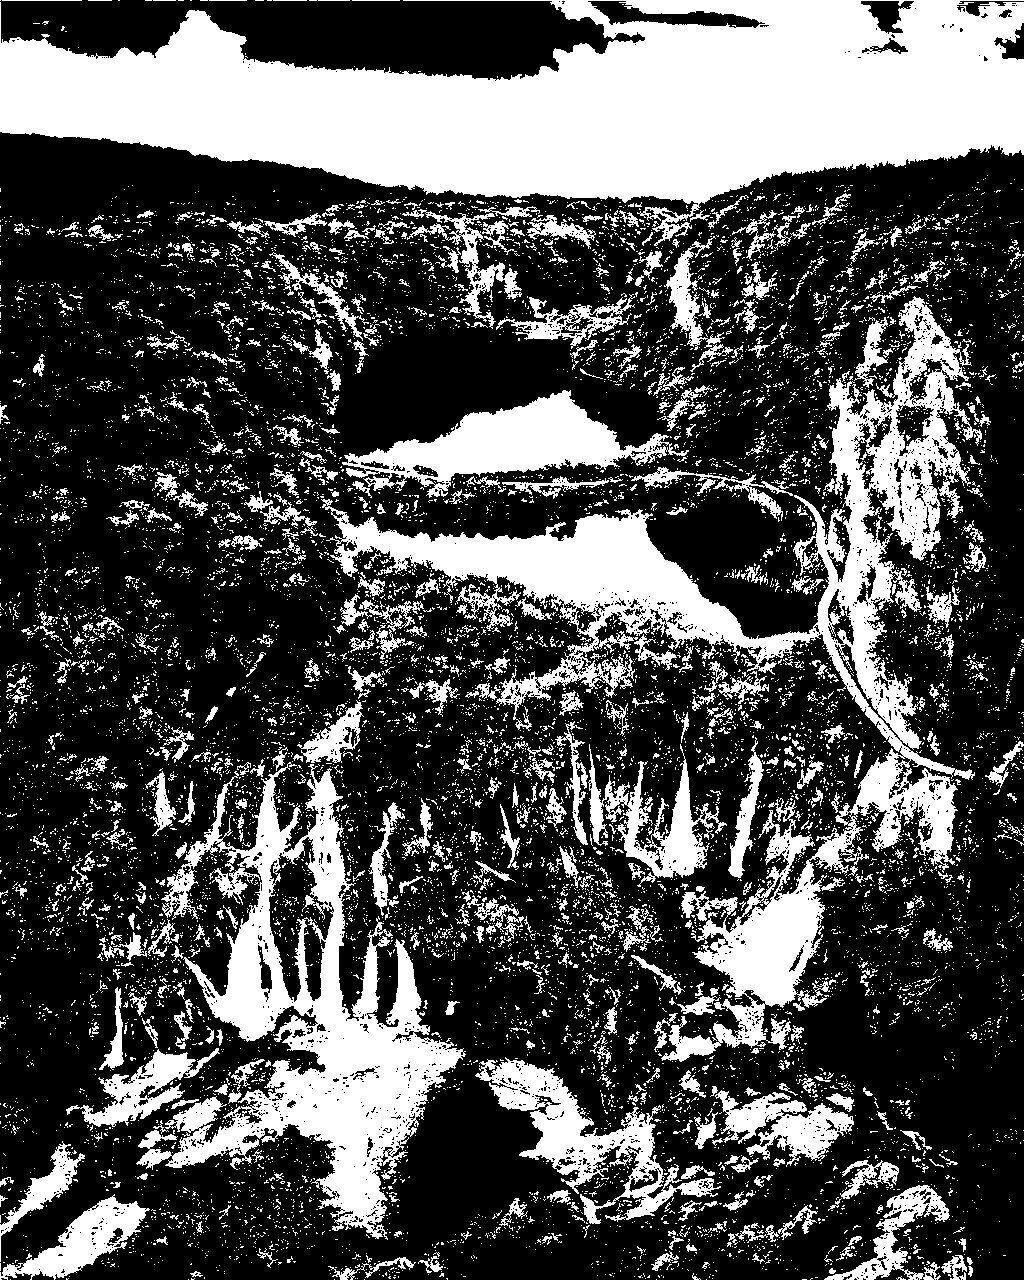
\includegraphics[width=0.75\linewidth]{slike/Binary.jpeg}
    \caption{Prikaz binarne slike (vlastita izrada)}
\end{figure}


Sam proces izrade binarne slike je dosta jednostavan. Za početak potrebno je imati sivu sliku. Zatim se definira granica (\textit{eng. threshold}) u obliku postotka. Ta granica se zatim koristi za određivanje vrijednosti piksela, ako je vrijednost iznad granice onda se vrijednost postavlja na jedan, a inače na nulu. Priložena formula prikazuje osnovni tip kreiranja binarne slike (\textit{eng. tresholding}).

{\large
    \[
I_{\text{gray}}(x, y) = 0.299 \cdot R(x, y) + 0.587 \cdot G(x, y) + 0.114 \cdot B(x, y)
\]

\[
I_{\text{binary}}(x, y) =
\begin{cases}
1, & \text{if } I_{\text{gray}}(x, y) \geq T \\
0, & \text{if } I_{\text{gray}}(x, y) < T
\end{cases}
\]}


\subsection{Važnost različitih tipova digitalnih slika}

Do sada smo prošli kroz 3 najvažnija tipa digitalnih slika za ovaj rad. Kroz ovu cjelinu prikazat će se važnost pojedinog tipa slike naspram ostalih.

Zapravo najveća razlika između ovih tipova je broj kanala boje. Slike u boji imaju 3 kanala za razliku od sivih i binarnih slika koje imaju po jedan kanal. To zapravo znači da slike u boji sadrže značajno više informacija. 

No ponekad nam te informacije nisu potrebne ovisno o problemu koji pokušavamo riješiti. Na primjer ako pokušavamo detektirati boju svjetla na semaforu onda su nam informacije o bojama izrazito važne. No ako pokušavamo pročitati tekst sa prometnog znaka onda nam informacija o boji znaka i teksta ne doprinosi značajno rješavanju problema. Zapravo nam otežava rješavanje problema pošto moramo raditi sa nepotrebnim informacijama.

\begin{figure}[H]
    \centering
    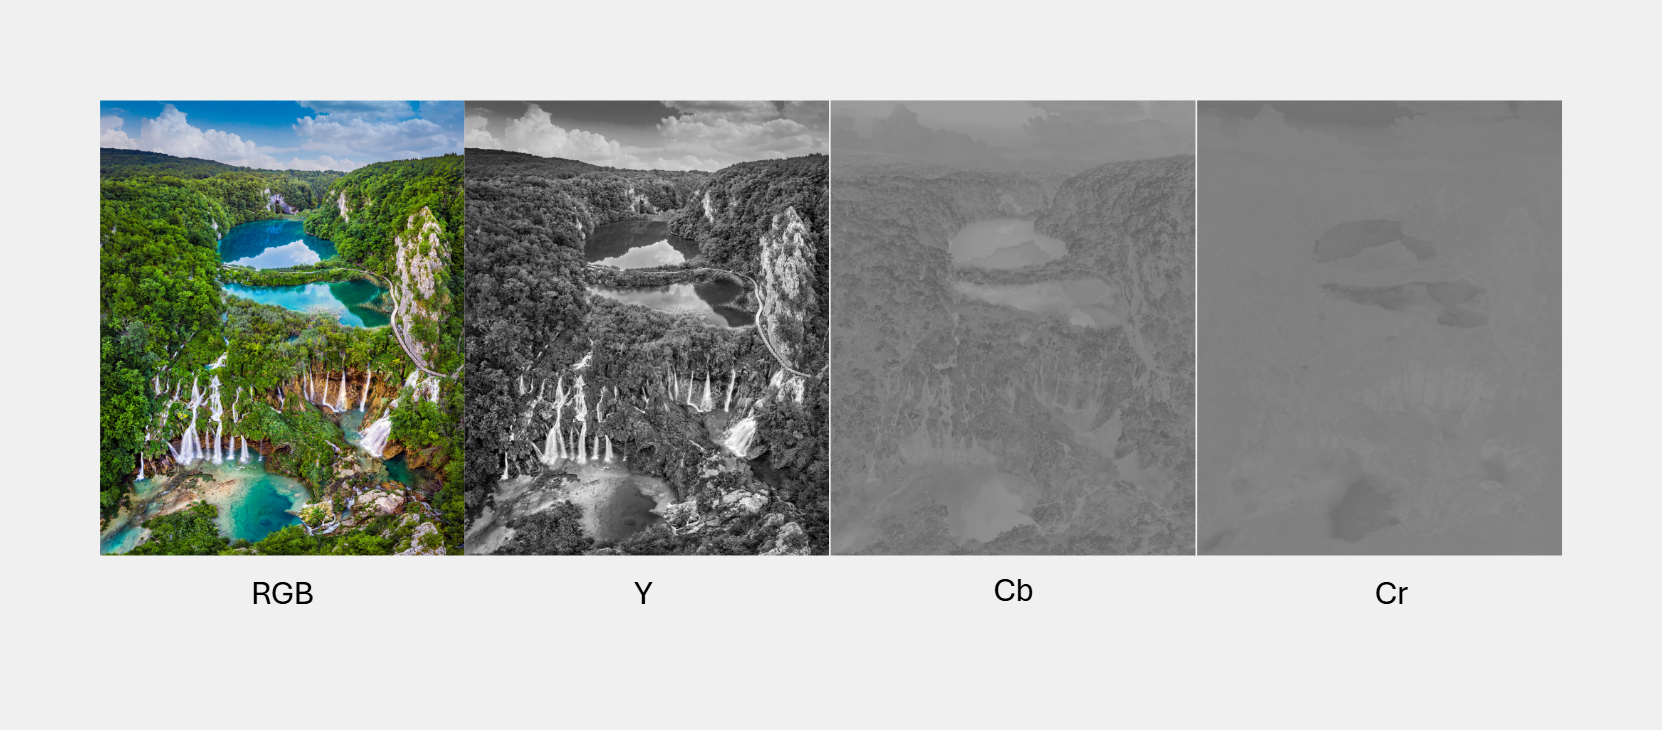
\includegraphics[width=1.0\linewidth]{slike/Luminace vs chrominance.png}
    \caption{Usporedba svjetlosne komponente i komponenta boja(vlastita izrada)}
\end{figure}

\begin{flushleft}
    Na priloženoj slici prikazana je ista slika na različite načine:
    \begin{itemize}[label=•]
        \item Slika u RGB formatu
        \item Slika u YCbCr formatu
        \begin{itemize}[label=•]
            \item Svjetlosne informacije u Y kanalu
            \item Informacije o bojama u Cb i Cr kanalima
        \end{itemize}
    \end{itemize}
    \end{flushleft}

Na ovom primjeru je prikazana činjenica da svjetlosni kanali sadrže puno više informacija o strukturnim elementima na slici. baš zbog toga se u raznim algoritmima za detektiranje značajki, filtriranje, segmentiranje i sl. koriste baš sive slike \cite{LumVsChrom}. 

Sive slike se koriste kada boja nije važan faktor u obradi slike. U tom slučaju je boja jednako korisna kao buka na slici pa je zbog toga uklonimo. Time se veličina slike smanje i time ubrza daljnji proces obrade slike \cite{LumVsChrom}.

Ako je potreban još agresivniji pristup otklanjanju nepotrebnih podataka onda binarne slike mogu postati korisne. One dodatno odstranjuju nepotrebne podatke tako da povećavaju razliku u kontrastu \cite{LumVsChrom}.

Važno je napomenuti da svaki tip slika ima svoju upotrebu ovisno o problemu koji se rješava. U ovom radu će veliku važnost imati sive i binarne slike pošto se radi o procesu detektiranja strukture fotografije i izvlačenja relevantnih informacija iz nje.


\section{Digitalna obrada slike}

Digitalna obrada slike (\textit{eng. digital image processing}) podrazumijeva obradu digitalne fotografije koristeći računalne algoritme s ciljem unaprjeđivanja slike, izvlačenja korisnih informacija i sl. Predstavlja ključni korak u raznim primjenama računalnog vida temeljenog na dubokom učenju, poput prepoznavanja lica, detekcije objekata i kompresije slika \cite{ImageProcessing}. 

\begin{flushleft}
Sam proces digitralne obrade slike može se podijeliti u sljedeće faze \cite{ImageProcessing}:
\begin{itemize}
\item Pribavljanje slike (\textit{eng. image acquisition})
\item Poboljšanje slike (\textit{eng. image enhancement})
\item Restauracija slike (\textit{eng. image restoration})
\item Kompresija slike (\textit{eng. image compression})
\item Morfološka obrada (\textit{eng. morphological processing})
\item Segmentacija slike(\textit{eng. image segmentation})
\item Reprezentacija i opis (\textit{eng. representation and description})
\item Detekcija i prepoznavanje objekata (\textit{eng. object detection and recognition})
\end{itemize}
\end{flushleft}

Naravno nisu sve faze uvijek potrebne, već se radi o generalnim smjernicama koje se prema specifičnostima problema mogu modificirati, smanjiti ili proširiti. U nekim slučajevima čak se redoslijed faza može promijeniti ili se faze mogu provoditi više puta.    

Te faze se dodatno podijeliti na \textbf{pretprocesiranje, procesiranje i postprocesiranje slike}. U fazu \textbf{pretprocesiranja} spadaju svi koraci koji pripremaju sliku za procesiranje, poput poboljšanja slike. Nakon pretprocesiranja slijedi \textbf{procesiranje} koje se odnosi na korištenje algoritama za detekciju i prepoznavanje objekata i transformacije. Posljednja faza uključuje korake poput pripreme rezultata za prezentaciju, vizualizaciju i daljnju analizu \cite{IamgeProcesingPhases}.

\pagebreak
\subsection{Pretprocesiranje slike}

Pretprocesiranje slike je ključan proces koji se provodi prije obrade slike. Kao ulaz prima izvornu, sirovu sliku, a kao izlaz vraća sliku u korisnijem formatu za daljnju obradu i analizu. Omogućuje da se sa slike odstrane ili istaknu područja relevantnih informacija te da se poboljša kvaliteta slike prije daljnje obrade \cite{Patel2023Oct}.


\subsubsection{Pribavljanje slike}

Pribavljanje slike je proces nastajanja digitalne slike tako da se informacije iz realnog svijeta zapiše u digitalnom obliku kojim računalo zatim može manipulirati. Slika se može pribaviti raznim uređajima poput fotoaparata, pametnog mobitela ali i drugih tehnologija poput skenera, rendgena i drugih uređaja. U ovom radu fokus će biti na fotografije probavljene uređajima koji posjeduju digitalnu kameru \cite{BibEntry2025Apr}.


Da bi bilo kakav procesiranje moglo krenuti prvo je potrebno pribaviti sliku. Moglo bi se reći da je pribavljanje slike čak najvažniji korak u cijelom procesu obrade slike, njegov rezultat ima veliku ulogu za postizanje krajnjeg rezultata obrade i analize slike. Pribavljena slika mora biti kvalitetna da bi ostali koraci bili uspiješni. Na kvalitetu slike ne utiječe samo rezolucija, osvjetljenje i kut pod kojim je slika uslikana također imaju značajnu ulogu \cite{BibEntry2025Apr}.

Razni algoritmi i koraci u pretprocesiranju mogu korigirati pribavljenu sliku, no to nikad nije zamjena za sliku dobre kvalitete. Dobra i loša slika mogu biti razlika između uspješnog i neuspješnog detektiranja elemenata na slici. Naravno u većini slučajeva sustavi za obradu slike ne mogu utjecati na kvalitetu slike koje će im korisnik poslati. Zbog toga je važno detaljno testirati sustav u različitim uvjetima i utvrditi što su njegove granice i je li potrebno podržati neki dodatni korisnički slučaj od onih postojećih.
\subsubsection{Poboljšanje slike}

Poboljšanje slike je ključan korak, cilj mu je modificirati sliku na način da ona postane korisnija za daljnu obradu. To se može postići na više načina poput otklanjanja buke, isticanja važnih značajki slike, poboljšanja oštrine i kontrasta slike.

Do sada smo spomenuli da se nepotrebene inforamcije na slici također mogu biti buka. Baš zbog toga pretvaranje u sivu i binarnu sliku spadaju pod poboljšanje slike. Oba dvije operacije uklanjaju nepotrebne inforamcije o bojama sa slike što omogučuje bržu i jednostavlniju obradu i analizu slike. naravno to ima smisla samo ako nam inforamcije o bojama nisu potrebene.

Osim nepotrebnih boja, bukom se može smatrati i nasumična razlika u boji između susjednih piksela. U digitalnoj fotografiji buka je praktički neizbježna i može se definirati kao nasumična varijacija signala u slici. Ta varijacija je reperezentirana različitim nijansama boja susjednih piksela. Buka se može smanjiti manipulacijom parametara digtalne kamera, ali ne može se kompletno ukoniti \cite{Adobe}.

Takve informacije se zbog malih razlika u boji piskela većinom mogu smatrati nevažnima, a loše utiječu na daljnu obradu slike. Zbog toga postoje razne tehnike za filtriranje slike. Najpopularnije tehnike za filtriranje buke su \cite{Swain2023Jul}:

\begin{itemize}
    \item Gaussov filter (\textit{eng. gaussian filter})
    \item Srednji filter (\textit{eng. mean filter})
    \item Medijanski filter (\textit{eng. median filter})
    \item Bilateralni filter (\textit{eng. bilateral filter})
\end{itemize}


Svaki tip filtera ima svoju upotrebu i koristan je za određeni tip buke. Buka u digitalnim slikama je jako opširna tima koje se neće detaljnije objašnajvati u ovom radu.

\begin{figure}[H]
    \centering
    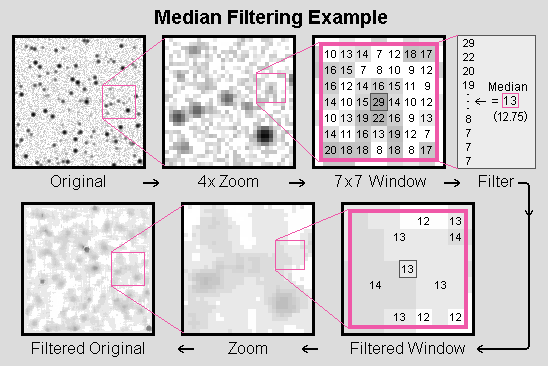
\includegraphics[width=1.0\linewidth]{slike/MedianFiltering.png}
    \caption{Primjer medijaskog filtera \cite{MeidanFilter}}
\end{figure}

Na priloženoj slici je prikazan proces korištenja medijanskog filtera koji naspram matrice susjednih vrijednosti određuje vrijednost piksela koristeći medijan svih vrijednosti. 

Važno je napomenuti da su pojmovi poput oštrine i mutnoće  slike usko povezani s bukom. Jako često mutna slika sadrži manje buke, dok oštra slika može sadržavati više buke. Zbog toga je potrebno naći ravnotežu pri uklanjanjanju buke. Ako uklonimo previše buke, slika postaje mutna i gubi se previše informacija, obrnuto vrijedi ako uklonimo premalo buke.

Postoji još razne metode poboljšavanja slike poput povećavanja kontrasta, ali neće biti potrebne u ovom radu.

\subsubsection{Restauracija slike}
Korištenje algoritama za rekonstrukciju oštećenih ili degradiranih dijelova slike.

\subsection{Procesiranje slike}
\begin{itemize}
    \item Ekstrakcija značajki i identifikacija struktura unutar slike
\end{itemize}

\subsubsection{Segmentacija slike}
Proces dijeljenja slike u regije koje predstavljaju različite objekte ili strukture.

\subsubsection{Morfološka obrada}
Primjena morfoloških operacija (dilatacija, erozija, otvaranje, zatvaranje) za poboljšanje strukture objekata na slici.

\subsubsection{Reprezentacija i opis}
Opis kontura, oblika i teksture objekata radi klasifikacije i analize.

\subsubsection{Detekcija i prepoznavanje objekata}
Otkrivanje i identifikacija objekata od interesa unutar slike. Uključuje:
\begin{itemize}
    \item \textbf{Detektiranje kontura} identifikacija granica objekata u slici.
    \item \textbf{Detektiranje linija} prepoznavanje pravaca pomoću metoda poput Houghove transformacije.
\end{itemize}

\subsection{Postprocesiranje slike}
\begin{itemize}
    \item Završna faza koja se odnosi na pohranu, vizualizaciju ili daljnju analizu rezultata.
\end{itemize}

\subsubsection{Kompresija slike}

\subsubsection{Vizualizacija rezultata}
Prikaz konačnih rezultata analize slike u svrhu interpretacije, izvještavanja ili donošenja odluka.

\section{Analiza postojećih rješenja i pristupa problemu}

\chapter{Praktični dio}
\section{Opis rješenja}
\section{Funkcionalni zahtijevi}
\section{Implementacija}
\section{Analiza rezultata}
\section{Limitacije riješenja}
\section{Manualno testiranje rješenja}
\chapter{Zaključak}


\printbibliography[title=Popis literature]
\addcontentsline{toc}{chapter}{Popis literature}

\listoffigures
\addcontentsline{toc}{chapter}{Popis slika}
 
\listoftables
\addcontentsline{toc}{chapter}{Popis popis tablica}

\appendix
\renewcommand{\thechapter}{\arabic{chapter}}


\end{document}
